\documentclass{beamer}
\useoutertheme[subsection=false]{miniframes}

\title{Game Theory project}
\author{Jagdev Bal, Ellie Fadipe, Jade Jones, Alex Room}
\date{4th of May, 2023}

\begin{document}
\begin{frame}
\titlepage
\end{frame}


\section{Introduction}
% Introduce insider trading
\begin{frame}{Introduction}

\end{frame}

% Introduce our investigation
\begin{frame}{Introduction}
    
\end{frame}


\section{Methods}
% Introduce notation and game model
\begin{frame}{Stage Game}
    
\end{frame}

% describe information and strategies
\begin{frame}{Information \& Strategy}
    
\end{frame}

\begin{frame}{Information \& Strategy}
    
\end{frame}

% describe the paired Moran process
\begin{frame}{Paired Moran Process}
Let $P_1$, $P_2$ be two populations; one of row players, and one of column players. Then the paired Moran process algorithm begins:
\begin{itemize}
\item Calculate the fitness of each member of each population against the \emph{other} population.
\item Birth and death for each population is then calculated from these fitnesses in the same way as the regular Moran process. This is done independently for each population.
\item Repeat until each population is homogeneous.
\end{itemize}

\end{frame}

\begin{frame}{Why?}
\begin{itemize}
    \item Information sets are uneven
    \item Populations don't interact within themselves
    \item Strategies don't 'carry over'
\end{itemize}
\end{frame}


\section{Results}
% co-winners heatmap
\begin{frame}{Co-Winners}
\begin{figure}[!h]
    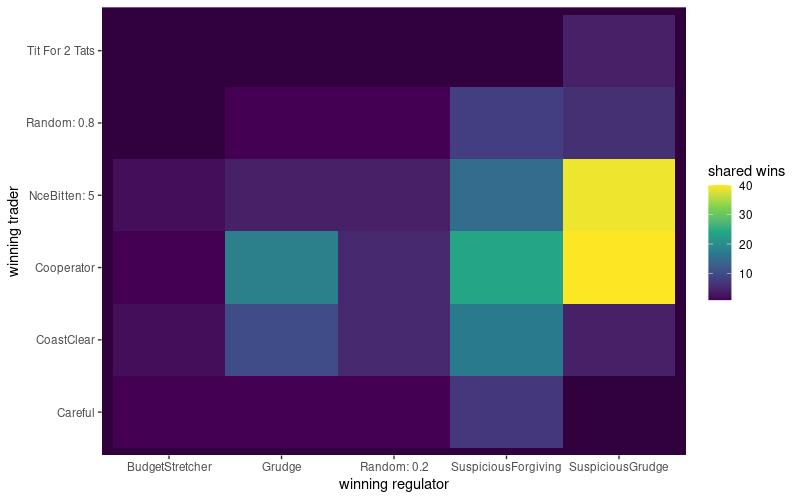
\includegraphics[width=\textwidth]{heatmap.png}
    \caption{A heatmap of co-winning trader-regulator pairs}
    \label{fig:f1}
\end{figure}
\end{frame}

% strategy survival for traders
\begin{frame}{Strategy Survival}
\begin{figure}[!h]
    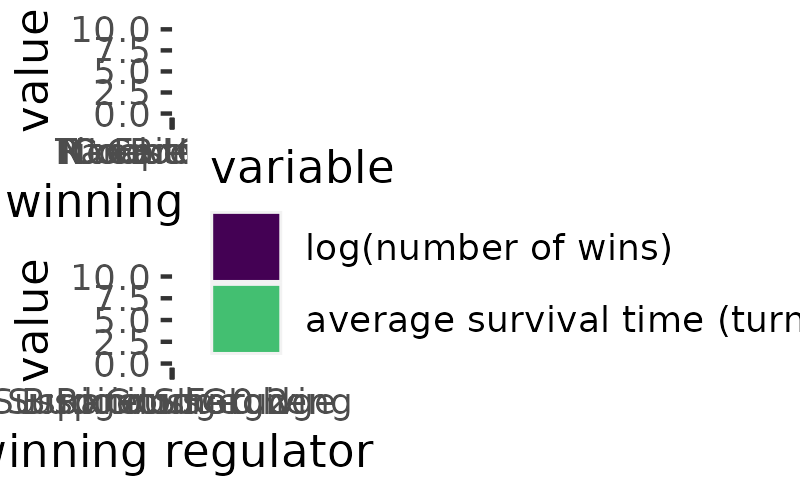
\includegraphics[width=\textwidth]{barplot.png}
    \caption{The number of wins (log base 10) and average survival time (in turns) of each trader/regulator}
    \label{fig:f2}
\end{figure}

\end{frame}

% strategy survival for regulators
\begin{frame}{Strategy Survival}
    
\end{frame}


\section{Conclusions}
% conclusions on data
\begin{frame}{Conclusions: Data}
    
\end{frame}

% conclusions on algorithms
\begin{frame}{Conclusions: Algorithm}
    
\end{frame}



\end{document}
